\section{Leaky bucket, pregi e difetti}

Quando ci si scambia pacchetti nella rete, serve un modo per controllare il flusso; per delimitare banda e velocità di trasmissione si può utilizzare l'algoritmo leaky bucket, un sistema di accodamento a singolo server con tempo di servizio costante.
\subsection{Cos'è?}
Questo algoritmo si basa sull'idea del “secchio che perde” attraverso il quale qualsiasi quantità d'acqua contenuta fluirà all'esterno sempre con la stessa velocità, se l'acqua viene aggiunta troppo velocemente questa supererà in volume la capacità del secchio e straborderà.

Allo stesso modo il leaky bucket è formato da una coda finita. Al suo arrivo, se c'è spazio il pacchetto viene aggiunto alla coda, altrimenti viene scartato. I pacchetti che sono in coda, vengono trasmessi uno alla volta ogni ciclo di clock (se la coda non è vuota). In questo modo si crea un flusso costante di pacchetti a differenza di un flusso casuale, cosi' da limitare congestioni causate dall'invio rapido di molti pacchetti.

\begin{figure}[H]
\centering
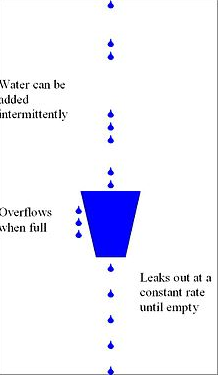
\includegraphics[scale=0.7]{res/img/41_LeakyBucket.png}
\end{figure}

\subsection{Pregi}
Burst di dati che potrebbero congestionare la rete vengono catturati dall'algoritmo che li distribuisce equamente.

\subsection{Difetti}
Ampie porzioni di risorse di rete non verranno utilizzate quando il volume del traffico è molto basso.\\
Quando la coda si riempie troppo i pacchetti in eccesso vengono brutalmente scartati.

\subsection{Ambiti d'uso}
Strato Network. Utilizzato nelle reti a commutazione di pacchetto, per controllare che le trasmissione dei pacchetti siano ben delimitati in banda e velocità di trasmissione.

\section{Descrivere il token bucket, pregi e difetti}

Per gestire il flusso di pacchetti su una rete è necessario utilizzare algoritmi che permettano un controllo della congestione e che sfruttino al meglio le risorse di rete. L'algoritmo leaky bucket (secchio che perde) gestiva le congestioni, ma purtroppo imponeva un modello di output troppo rigido, che non seguiva la variabilità del traffico.

Per molte applicazioni è meglio permettere all'output di accelerare un po' quando ci sono burst di dati, perciò serve un algoritmo più flessibile e che non perda mai dati.
\subsection{Cos'è?}
L'algoritmo token bucket riprende l'idea del leaky bucket, ma aggiunge dei token, generati da un clock.
Un pacchetto per passare deve distruggere un token, se non c'è, attende finché non viene generato dal clock. A differenza del leaky bucket, il token bucket non scarta i pacchetti quando il secchio è pieno.

Se non arrivano pacchetti da inviare, il token bucket accumula i token fino ad un massimo di n. Così facendo si prepara a gestire dei possibili burst di massimo n pacchetti (pari al numero di token), bruciando i token in rapida successione e dando una risposta più veloce a picchi improvvisi.

Per implementare questo algoritmo è necessaria solo una variabile che tenga conto del numero di token, e li diminuisca quando un pacchetto viene inviato.

\begin{figure}[H]
\centering
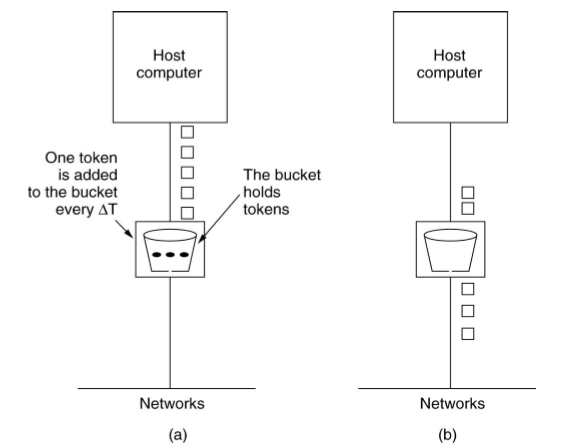
\includegraphics[scale=0.6]{res/img/42_TokenBucket.png}
\end{figure}
 
\subsection{Pregi}
Al contrario del leaky bucket, usando quest'algoritmo non scarta nessun pacchetto.\\
Gestisce meglio i burst improvvisi, dando una risposta più veloce.
\subsection{Difetti}
Un potenziale difetto può essere che consente di trasmettere grandi raffiche di dati, che potrebbero causare congestione. (non sicura).
\subsection{Ambiti d'uso}
Strato Network, utilizzato per gestire il traffico in una rete dati, finalizzato a regolare l'output di trasmissione.

\section{Descrivere l'ARP}
Ogni macchina di Internet ha uno o più indirizzi IP, tuttavia questi non possono essere utilizzati per inviare pacchetti, in quanto l'hardware che opera sullo strato data link non comprende gli indirizzi Internet.
Bisogna trovare un modo per associare l'indirizzo Ethernet a 48 bit (indirizzo MAC) con l'indirizzo IP associato.
\subsection{Cos'è?}
ARP è un protocollo che permette di associare un indirizzo IP all'indirizzo Ethernet in una sottorete (o anche tra più sottoreti utilizzando Arp-proxy).
Viene trasmesso un pacchetto broadcast a tutte le stazioni nella sottorete che chiede chi è il proprietario di un determinato indirizzo IP. Le stazioni controllano il proprio indirizzo IP e solo il proprietario di tale indirizzo risponde inviando il proprio indirizzo Ethernet. In questo modo la stazione che cercava un determinato indirizzo riesce a collegare l'IP con il MAC.

A questo punto, il software IP costruisce un frame Ethernet indirizzato al destinatario appena scoperto e inserisce il pacchetto IP nel campo carico utile, dopodiché scarica tutto sulla Ethernet. 
La scheda Ethernet del destinatario rileva il frame, si accorge di essere la stazione designata della comunicazione, preleva i dati ed estrae il pacchetto IP dal carico utile per passarlo al software IP, il quale verifica la correttezza dell'indirizzo ed elabora i dati.
Per migliorare le prestazioni, dopo aver associato degli indirizzi, questi vengono memorizzati nella cache, così, in caso di nuove trasmissioni verso la stessa stazione, si ha già l'indirizzo pronto.

Il vantaggio dell'ARP e' la sua semplicita': il sistemista non deve fare altro se non assegnare un indirizzo IP al terminale (oppure eseguita dal DHCP). ARP si occupa del resto.

\begin{figure}[H]
\centering
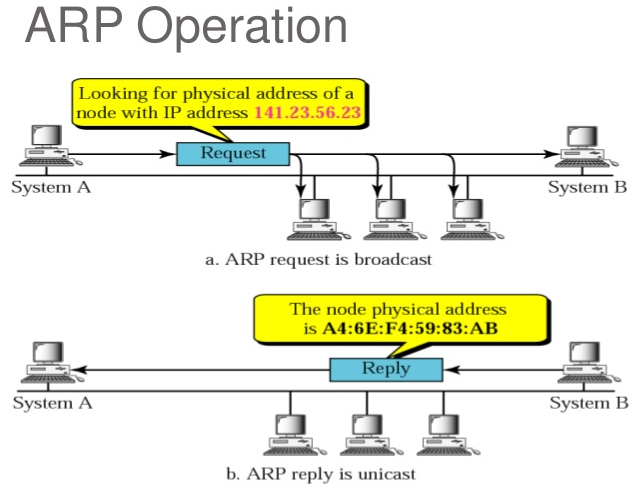
\includegraphics[scale=0.6]{res/img/43_ARP.png}
\end{figure}
\subsection{Pregi}
Permette la trasmissione di pacchetti ad un host anche senza conoscere l'indirizzo MAC (necessario per instaurare una connessione a livello data-link).
\subsection{Difetti}
Non autentica le risposte, il che lo rende molto vulnerabile a possibili attacchi.

\subsection{Ambiti d'uso}
Utilizzato nel protocollo IPv4 e operante a livello di accesso alla rete. \\
Viene utilizzato tutte le volte che un host collegato ad una LAN deve inviare un messaggio ad un host nella stessa LAN conoscendo solamente l'indirizzo IP.

\section{Si descriva DHCP e il suo funzionamento}

Con ARP è possibile associare (in una sottorete) l'indirizzo MAC di una macchina conoscendo il suo indirizzo IP.
A volte è necessario risolvere il problema inverso: dato un indirizzo Ethernet, qual è il corrispondente indirizzo IP?

È stato creato una possibile soluzione, RARP, che permette di risolvere il problema, tuttavia necessita di installare su ogni router dei server RARP. Per aggirare questo problema si è passati ad un protocollo alternativo BOOTP, che a differenza di RARP utilizza messaggi UDP inoltrati attraverso i router. Purtroppo, questo protocollo necessita una configurazione manuale delle tabelle che associano indirizzi IP e agli indirizzi Ethernet (non è possibile utilizzare BOOTP fino a quando l'amministratore non assegna alla macchina un indirizzo IP e non inserisce manualmente l'associazione del tipo nelle tabelle di configurazione di BOOTP).

Per risolvere questo problema BOOTP viene esteso e chiamato in modo diverso, cioè DHCP (Dynamic Host Configuration Protocol), che permette un'assegnazione manuale o automatica degli indirizzi IP.
Questo protocollo ha ampiamente sostituito RARP e BOOTP.

\subsection{Cos'è?}
DHCP si basa sull'idea di un server speciale che assegna gli indirizzi IP agli host che ne richiedono uno.
Questo server non deve trovarsi sulla stessa LAN, il che comporta che potrebbe non essere raggiunto dalle trasmissioni broadcast, perciò è necessario installare in ogni LAN un agente di inoltro DHCP.

Una macchina appena accesa invia in modalità broadcast un pacchetto DHCP DISCOVER; questo pacchetto viene intercettato dall'agente di inoltro presente nella LAN che provvede ad inoltrarlo al server DHCP che assegna un indirizzo IP alla macchina tramite un pacchetto DHCPOFFER, questa risponde con un pacchetto DHCPREQUEST che viene accettata dal server tramite ACK.
Questo avviene nel caso di un singolo server DHCP, potrebbero essercene multipli, in questo caso l'host che necessita di un indirizzo IP valuta le varie proposte, ed invia un pacchetto DHCPREQUEST indicando il server selezionato.
L'indirizzo assegnato proviene da una pool di indirizzi IP comuni, un problema causato da questo potrebbe essere la durata di allocazione: se un host abbandona la rete senza restituire l'indirizzo IP questo viene perso per sempre.

Per evitare questa eventualità, gli indirizzi IP sono assegnati secondo una tecnica chiamata di leasing, ovvero a scadenza di tempo. Prima che questo scada l'host deve fare richiesta di rinnovo dell'indirizzo, se non riesce a farla o se viene rifiutata, l'host non può più utilizzare quell'indirizzo IP.

\begin{figure}[H]
\centering
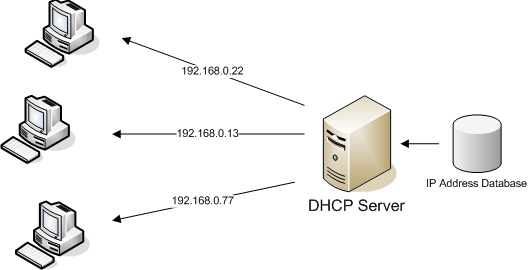
\includegraphics[scale=0.6]{res/img/44_DHCP.png}
\end{figure}

\subsection{Pregi}
Permette di associare indirizzi IP avendo l'indirizzo MAC di un'host.

\subsection{Difetti}
Non include nessun meccanismo di autenticazione, il che lo rende vulnerabile a possibili attacchi

\subsection{Ambiti d'uso}
Protocollo di rete a livello applicativo, utilizzato ampiamente nelle reti odierne.

\section{IPV6}

Un indirizzo IP, è un'etichetta numerica che identifica univocamente un dispositivo (host) collegato ad una rete informatica che utilizza l'Internet Protocol come protocollo di rete.

IPv4 (Internet Protocol version 4) è attualmente il protocollo più usato a livello di rete, la sua tecnologia però supporta al massimo $2^32$ indirizzi univoci.
Inizialmente poteva andare bene, ma con la crescita esponenziale della rete questi iniziano a scarseggiare. Esistono protocolli tipo CIDR e NAT che permettono di sfruttare gli indirizzi IP restanti in modo variabile, così da resistere ancora un po', tuttavia IPv4 ha i giorni contati.

IPv6 è un upgrade dell'IPv4 e conta di risolvere i problemi di numero, in quanto riuscirebbe a gestire $2^128$ indirizzi diversi.
IPv6 oltre a colmare il problema della quantità di indirizzi migliora e semplifica l'intestazione: infatti prevede solo 8 campi rispetto ai 13 dell'IPv4. Questo consente al router di elaborare i pacchetti più velocemente. Sempre riguardo l'elaborazione dei pacchetti, IPv6 migliora il supporto per le opzioni, rendendo campi che prima erano obbligatori, opzionali. Un altro grande passo avanti riguarda la sicurezza. E' stata anche data importanza anche al quality of service.

IPv6 e IPv4 non sono compatibili tra loro, ma rimane compatibile con una varieta' di protocolli quali TCP, UDP, ICMP etc. \\Tuttavia la rete ormai è basata sull'IPv4 e il passaggio alla versione successiva è lenta e impegnativa, si stanno facendo passi avanti, però rimane la necessità di mantenere entrambi i protocolli almeno per decenni prima di passare alla nuova versione.

\begin{figure}[H]
\centering
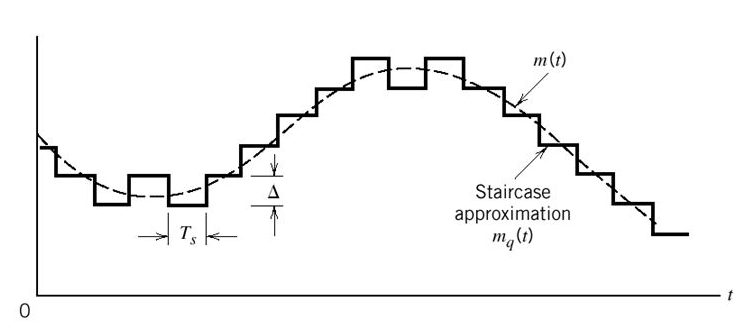
\includegraphics[scale=0.6]{res/img/6_modulazioneDelta.png}
\end{figure}

\subsection{Pregi}
Aumenta di molto gli indirizzi gestibili rispetto all'IPv4.\\
Migliora e semplifica l'intestazione, consentendo una elaborazione di pacchetti più veloce.\\
Migliora il supporto per le opzioni e migliora la sicurezza.

\subsection{Difetti}
Non è compatibile con il predecessore, quindi l'introduzione a questo nuovo protocollo è lenta.

\subsection{Ambiti d'uso}
Protocollo di rete, utilizzato per gli indirizzi di rete.

\section{Elencare e descrivere brevemente i secondi (primi) 32b dell'header IPv4 (IPv6)}
(sinceramente sta domanda non la capisco… faccio entrambe le versioni, poi nella risposta va scelta quella che viene richiesta. inizio con un'intro comune, poi un'intro per IPv4 e una IPv6 (da scegliere), successivamente descrivo in blocco i primi 32b dell'IPv4, seguiti dai secondi 32, poi faccio lo stesso per IPv6, Enjoy).\\

Un indirizzo IP, è un'etichetta numerica che identifica univocamente un dispositivo (host) collegato ad una rete informatica che utilizza l'internet Protocol come protocollo di rete.\\
\subsection{IPv4}
\textbf{IPv4} è il protocollo più usato e la sua tecnologia può supportare al massimo $2^32$ indirizzi univoci, numero che sta iniziando a diventare stretto.
Un datagramma IP di questa versione è costituito da una parte di intestazione e una parte di testo. L'intestazione è di 20B fissi e una parte opzionale di lunghezza variabile, consiste in 13 campi.\\
\subsection{IPv6}
\textbf{IPv6} è l'evoluzione dell'IPv4 e conta di risolvere molti dei suoi problemi, può supportare al massimo $2^128$ indirizzi univoci.
Un datagramma IP di questa versione è costituito da una parte di intestazione e una parte di carico utile. L'header è costituito dai primi 40 byte e contiene 8 campi, il carico utile invece va da un minimo di 1280 byte e arriva fino a 65535 byte (in modalità standard).

\subsection{IPv4, primi 32bit}
\begin{itemize}
\item	Version [4 bit]: indica la versione del pacchetto IP; per IPv4, ha valore 4.
\item	Internet Header Lenght (IHL) [4bit]: indica la lunghezza (in word da 32 bit) dell'header del pacchetto IP; tale lunghezza può variare da 5 word (20 byte) a 15 word (60 byte) a seconda della presenza e della lunghezza del campo facoltativo.
\item	Type of Service (TOS) [8 bit]: Nelle specifiche iniziali, questo campo avrebbe dovuto specificare il modo e la precedenza con cui l'host ricevente doveva trattare il datagramma;
Ad esempio, un host poteva scegliere una bassa latenza, mentre un altro preferire un'alta affidabilità. Nella pratica questo uso del campo TOS non ha preso piede.
\item	Total Length [16 bit]: Indica la dimensione (in byte) dell'intero pacchetto, comprendendo header e dati.
\end{itemize}

\subsection{IPv4, secondi 32bit}
\begin{itemize}
\item	Identification [16 bit]: Inizialmente sarebbe dovuto essere utilizzato per identificare in modo univoco i vari frammenti in cui può essere spezzato un pacchetto IP. Sperimentazioni successive però hanno suggerito di utilizzarlo per aggiungere la funzionalità di tracciamento dei pacchetti. Serve per determinare quale datagramma appartiene al frammento appena arrivato (tutti i frammenti di un datagramma hanno lo stesso campo identification).
\item	Flags [3 bit]: Bit utilizzati per il controllo del protocollo e della frammentazione dei datagrammi. Il primo è Reserved sempre settato a “0” (bit inutilizzato in poche parole), successivamente troviamo DF (Don't Fragment) se settato a “1” indica che il pacchetto non deve essere frammentato, se non è possibile inviarlo senza frammentazione, il pacchetto viene scartato. L'ultimo bit di flag è MF (More Fragments) se settato a “0” indica che il pacchetto è l'ultimo frammento (o il solo frammento del pacchetto originario), perciò tutti gli altri frammenti dello stesso pacchetto avranno MF settato a “1”. 
\item	Fragment Offset [13 bit]: Indica l'offset (misurato in blocchi di 8 byte) di un particolare frammento relativamente all'inizio del pacchetto IP originale: il primo frammento ha offset 0, i successivi avranno valore multiplo di 8byte e indica la posizione del frammento nel datagramma. Il valore massimo è pari a 65536 byte.
\end{itemize}

\begin{figure}[H]
\centering
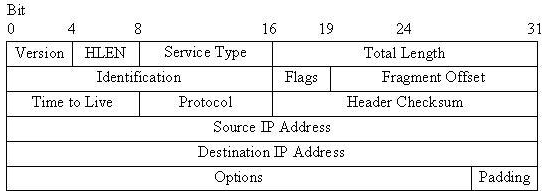
\includegraphics[scale=0.7]{res/img/46_IPv4.png}
\end{figure}

\subsection{IPv6, primi 32bit}
\begin{itemize}
\item	Version [4 bit]: Indica la versione del datagramma IP: per IPv6, ha valore 6 (lel).
\item	Traffic Class [8 bit]: Permette di gestire le code di priorità, assegnando ad ogni pacchetto una classe di priorità rispetto ad altri pacchetti provenienti dalla stessa sorgente. Viene usata anche per controllare la congestione.
\item	Flow Label [20 bit]: Campo ancora in fase sperimentale, usato dal mittente per etichettare una sequenza di pacchetti come se fossero nello stesso flusso. Supporta la gestione del QoS (Quality of Service) consentendo ad esempio di specificare quali etichette abbiano via libera rispetto ad altre. I pacchetti con flow label diverso da “0” avranno trattamenti speciali dai router.
\end{itemize}
\subsection{IPv6, secondi 32bit}
\begin{itemize}
\item	Payload Length [16 bit]: è la dimensione del payload (carico utile), ovvero il numero di byte di tutto il contenuto presente dopo l'header.
\item	Next Header [8 bit]: Indica quale tipo di processo di trasporto è in attesa di quei dati (UDP, TCP o altri). Simile al campo protocol dell'IPv4 con cui condivide i valori.
\item	Hop Limit [8 bit]: Indica il tempo di vita del pacchetto, il suo valore viene decrementato di 1 ogni volta che il pacchetto passa da un router, quando arriva a 0 viene scartato. Simile al campo Time to live presente nell'IPv4.
\end{itemize}

\begin{figure}[H]
\centering
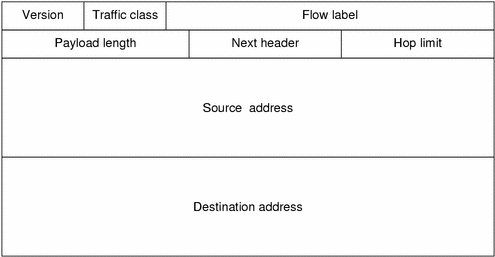
\includegraphics[scale=0.7]{res/img/46_IPv6.png}
\end{figure}

\textbf{NOTA:} Ripeto che questa domanda alla fine contiene 4(?) domande possibili, bisogna utilizzare i pezzi che vengono richiesti al momento, letta tutta d'un fiato non ha senso, è divisa e si dovrebbe capire il suo contenuto, se non lo capite cambiate esame :P

\section{Frame Ethernet}
\subsection{Cos'è?}
Un frame Ethernet è l'unità trasportata nel livello Data Link.
Esistono diverse versioni di questo frame; ora analizziamo la versione IEEE 802.3. 

Un frame Ethernet ha una grandezza compresa tra 64 e 1518 byte, ed è formato da:
\begin{itemize}
\item	Preambolo [7 byte]: contenente “10101010” e serve per sincronizzare il clock del ricevitore con quello del trasmettitore.
\item	SFD [1 byte]: Start of the Frame, “10101011” indica al destinatario che dal prossimo byte comincerà il frame vero e proprio.
\item	MAC address di destinazione [6 byte]: Indica l'indirizzo di destinazione, il bit di ordine più elevato vale “0” per gli indirizzi ordinari e “1” per quelli di gruppo. Con gruppo si intende una trasmissione multicast, che differisce dalla broadcast, più rozza ma che non richiede alcuna gestione. Per una trasmissione broadcast basta mettere tutti i bit a “1”.
\item	MAC address sorgente [6 byte]: indica l'indirizzo sorgente del frame.
\item	Type [2 byte]: Indica al ricevitore cosa deve fare del frame. Sullo stesso computer si possono usare più protocolli dello stato network contemporaneamente, questo campo indica il processo a cui passare il frame.
\item	Dati [da 46 a 1500 byte]: Questo campo contiene i dati veri e propri, non può essere nullo in quanto Ethernet richiede frame lunghi almeno 64 byte (dal destination address al checksum inclusi). Perciò se la parte occupata dai dati è lunga meno di 46 byte il campo successivo viene utilizzato per riempire il frame.
\item	Pad [0-46 byte]: Come descritto sopra, se il frame dati è inferiore a 46 byte, questo campo provvede a riempire i byte mancanti, cosi che vengano accettati dal protocollo Ethernet.
\item	Checksum [4 byte]: Contiene codice CRC per il rilevamento degli errori (senza correzione).
\end{itemize}

\begin{figure}[H]
\centering
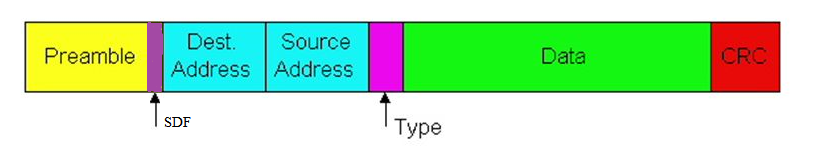
\includegraphics[scale=0.6]{res/img/47_FrameEthernet.png}
\end{figure}

\section{Si descriva l'header UDP}

Lo stato di trasporto è il cuore dell'intera gerarchia dei protocolli. Il suo compito è fornire il trasporto dei dati, affidabile ed efficiente in termini di costi, dal computer di origine a quello di destinazione, indipendentemente dalla rete o dalle reti fisiche effettivamente utilizzate.
Nello strato di trasporto ci sono due protocolli principali, che si distinguono dal fatto che uno è orientato alla connessione l'altro è senza connessione (TCP e UDP).\\
\textbf{Senza connessione:} lo scambio di dati a pacchetto tra mittente e destinatario non richiede l'operazione preliminare di creazione di un circuito su cui instradare l'intero flusso.
\subsection{Cos'è UDP?}
UDP (User Datagram Protocol) è un protocollo dello stato di trasporto senza connessione. Non gestisce il riordinamento dei pacchetti né la ritrasmissione di quelli persi, il che lo rendono di minor affidabilità rispetto al TCP. In compenso è molto rapido ed efficiente per applicazioni leggere o time sensitive (audio video real-time).
UDP fornisce servizi basilari: Multiplazione delle connessioni tramite assegnazione delle porte e verifica degli errori mediante una checksum inserita in un campo dell'header.
\subsection{Header UDP}
L'header dell'UDP è cosi formato:
\begin{itemize}
\item	Source port [16 bit]: identifica il numero di porta sull'host del mittente del datagramma;
\item	Destination port [16 bit]: identifica il numero di porta sull'host del destinatario del datagramma;
\item	Length [16 bit]: contiene la lunghezza totale (in byte) del datagramma UDP (header+dati);
\item	Checksum [16 bit]: contiene il codice di controllo del datagramma, l'algoritmo di calcolo è definito nell'RFC del protocollo (documento con informazioni e specifiche del protocollo).
\end{itemize}
Infine sono presenti i dati del messaggio.

\subsection{Pregi}
Rapido ed efficiente per applicazioni leggere e che necessitano di velocità di trasmissione.
\subsection{Difetti}
Non gestisce il riordinamento dei pacchetti e la ritrasmissione di quelli persi.\\
Non da nessuna affidabilità.
\subsection{Ambiti d'uso}
UDP viene utilizzato dalle applicazioni di rete che sono elastiche riguardo alla perdita dei dati e strettamente dipendenti dal tempo, si usa inoltre per comunicazioni in broadcast (tutti i terminali in una rete) e multicast (tutti i terminali iscritti ad un servizio).

\begin{figure}[H]
\centering
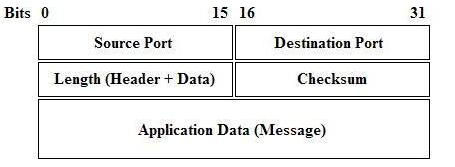
\includegraphics[scale=0.8]{res/img/48_HeaderUDP.png}
\end{figure}
 
\section{Descrivere l'header TCP/IP e commentarlo}
Lo stato di trasporto è il cuore dell'intera gerarchia dei protocolli. Il suo compito è fornire il trasporto dei dati, affidabile ed efficiente in termini di costi, dal computer di origine a quello di destinazione, indipendentemente dalla rete o dalle reti fisiche effettivamente utilizzate.
Nello strato di trasporto ci sono due protocolli principali, che si distinguono dal fatto che uno è orientato alla connessione l'altro è senza connessione (TCP e UDP).\\
\textbf{Orientato alla connessione}: I dispositivi utilizzano un protocollo di comunicazione per stabilire una connessione end-to-end tra gli agenti della comunicazione prima della trasmissione di qualsiasi tipo di dato.
\subsection{Cos'è TCP?}
\textbf{TCP} (Transmission Control Protocol) è il protocollo orientato alla connessione dello strato di trasporto. Si occupa di controllo della trasmissione, di rendere affidabile la comunicazione di dati in rete tra mittente e destinatario.

Contrariamente a UDP, TCP riesce a garantire la consegna dei dati, utilizzando meccanismi di acknowledgment e di ritrasmissione su timeout, al costo però di un maggior overhead (viene usata più banda di quello che servirebbe per i dati) della rete.
TCP inoltre possiede funzionalità di controllo di flusso e controllo della congestione (attraverso la sliding window).
TCP è solitamente usato in combinazione con il protocollo di livello di rete IP. Erroneamente TCP/IP sono considerati un unico protocollo.
\subsection{Header TCP}
L'header del TCP è formato nel seguente modo:
\begin{itemize}
\item	Source port [16 bit]: Identifica il numero di porta sull'host mittente associato alla connessione TCP.
\item	Destination port [16 bit]: Identifica il numero di porta sull'host destinatario.
\item	Sequence number [32 bit]: Indica lo scostamento (in byte) dell'inizio del segmento TCP interno al flusso completo, a partire dall'ISN (initial sequnce number), negoziato all'apertura della connessione.
\item	Acknowledgment number [32 bit]: Ha senso solo se il flag ACK è impostato a “1”, e conferma la ricezione di una parte del flusso di dati nella direzione opposta, indicando il valore del prossimo Sequence number che l'host mittente del segmento TCP si aspetta di ricevere.
\item	Data offset [4 bit]: Indica la lunghezza (in word da 32 bit) dell'header del segmento TCP; può variare in base alla presenza e alla lunghezza del campo facoltativo Options.
\item	Reserved [4 bit] Bit non utilizzati. Predisposti per sviluppi future dell'applicazione.
\item	Flags [8 bit]: Bit utilizzati per il controllo del protocollo:
\begin{itemize}
\item	CWR (Congestion Window Reduced): Se impostato a “1” indica che l'host sorgente ha ricevuto un segmento TCP con flag ECE (prossimo) impostato a “1”. 
QUESTA è NUOVA, NON CREDO SERVA
\item	ECN (Explicit Congestion Notification): se impostato a “1” indica che l'host supporta L'ECN durante il 3-way handshake. QUESTA è NUOVA, NON CREDO SERVA
\item	URG: Se impostato a “1” indica che nel flusso sono presenti dati URGENTI alla posizione (offset) indicata nel campo Urgent pointer.
\item	ACK: Se impostato a “1” indica che il campo Acknowledgment number è valido;
\item	PSH: Se impostato a “1” indica che i dati in arrivo devono essere passati subito ai livelli superiori senza che vengano bufferizzati.
\item	RST: Se impostato a “1” indica che la connessione non è valida; usato in caso di errore grave; Utilizzato per la reimpostazione della connessione diventata incongruente.
\item	SYN: Indica che l'host mittente del segmento vuole stabilire una connessione e specifica nel campo Sequence number il valore dell'ISN; utilizzato per stabilire le connessioni. Chi invia il SYN deve attendere dall'host remoto un SYN/ACK.
\item	FIN: Se impostato a “1” indica che l'host mittente del segmento vuole chiudere la connessione TCP aperta con l'host destinatario, chi invia FIN non può più inviare dati, mentre il destinatario ha ancora la linea aperta, dovrà inviare un ACK per chiuderla definitivamente.
\end{itemize}
\item	Window size [16 bit]: Indica la dimensione della finestra di ricezione dell'host mittente, cioè il numero di byte che il mittente è in grado di accettare a partire da quello specificato nell' Acknowledgment number.
\item	Checksum [16 bit]: Campo di controllo utilizzato per la verifica della validità del segmento. L'algoritmo di checksum somma semplicemente i complementi a uno delle parole di 16 bit e quindi calcola il complemento a uno della somma. Quando il ricevente esegue il calcolo sull'intero segmento (compreso il checksum) il risultato dovrebbe essere 0.
\item	Urgent pointer [16 bit]: Puntatore a dato urgente, ha senso solo se il flag URG è impostato a “1”, indica lo scostamento in byte a partire dal Sequence number del byte di dati urgenti all'interno del flusso.
\item	Options: opzioni facoltative per usi del protocollo avanzati.
\item	Data: Rappresenta il carico utile (payload) da trasmettere.
\end{itemize}

\begin{figure}[H]
\centering
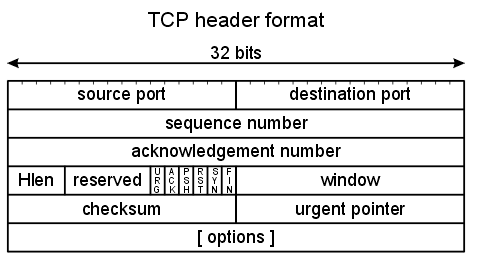
\includegraphics[scale=0.7]{res/img/49_HeaderTCP.png}
\end{figure}

\subsection{Pregi}
Possiede funzionalità di controllo di flusso e controllo della congestione (attraverso la sliding window).
Da grande affidabilità nel trasporto di pacchetti nella rete.

\subsection{Difetti}
Utilizza molta banda per fornire tutte le feature, feature che per molte applicazioni non sono utili, con conseguente spreco di banda nei loro casi.

\subsection{Ambiti d'uso}
Strato di trasporto, presente nei terminali. Implementato all'interno del sistema operativo. Usato nella stragrande maggioranza delle applicazioni internet che richiedono una consegna affidabile di pacchetti (che UDP non può garantire).

\section{Cos'è il DNS?}
\subsection{Cos'è?}
Protocollo dello strato applicativo, \textbf{DNS} (Domain Name System) è un sistema per la risoluzione di nomi degli host in indirizzi IP. 
L'essenza del DNS è l'invenzione di uno schema di denominazione gerarchico basato su dominio, e di un sistema di database distribuito per l'implementazione di questo schema di denominazione.

Per associare un nome ad un indirizzo IP, un programma applicativo chiama una procedura di libreria chiamata risolutore, passando il nome come parametro. Il risolutore invia un pacchetto UDP ad un server DNS locale, che quindi cerca il nome e restituisce l'indirizzo IP al risolutore, che a sua volta lo restituisce al chiamante. Ora il programma, conoscendo l'indirizzo IP, può stabilire una connessione TCP con la destinazione oppure inviarle i pacchetti UDP.

Questa tecnica è utile in quanto l'ampia diffusione di internet anche per utenti non tecnici non è pratica a memorizzare indirizzi IP numerici, per questo modificandoli in nomi testuali sono più semplici da memorizzare e utilizzare.

È possibile inoltre attribuire più nomi allo stesso indirizzo IP (o viceversa) per rappresentare diversi servizi o funzioni forniti da uno stesso host.
Una stringa come www.ciaofede.it indica un host a cui ti sei connesso e a sua volta può essere scomposto in tre segmenti distinti:
\begin{itemize}
\item	It denota il dominio di primo livello;
\item	Ciaofede è un dominio di secondo livello, cioè il nome che caratterizza questo sito web (insieme a .it).
\item	www è il dominio di terzo livello ed identifica un particolare host all'interno del dominio ciaofede.it.
\end{itemize}
Così facendo grazie al DNS è possibile visitare quell'host remoto senza dover scrivere l'indirizzo IP del server, ma scrivendo l'indirizzo testuale e facile da ricordare.

\begin{figure}[H]
\centering
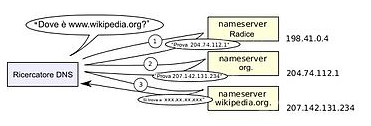
\includegraphics[scale=1]{res/img/50_DNS.png}
\end{figure}

\subsection{Pregi}
Garantisce una maggior chiarezza per l'utente medio.

\subsection{Difetti}
--
\subsection{Ambiti d'uso}
Strato Applicativo.\\
Utilizzato per la risoluzione di nomi della rete.\\
Utilizzato molto nei web server, in cui con un singolo indirizzo IP si possono ospitare più siti web.